\section{Test on real data}

We test the algorithm described above on a LOFAR dataset. The
visibilities produced by this interferometer are predominantly
affected by direction dependent effects including (i) the phased beam instability and deviation from the
theoritical model, (ii) ionosphere time delays shifts, and (iii)
Faraday rotation.

We first calibrate the data using BBS, and in order to build a
pertinent model of the field, we substract 3C295. We extract the
sources using pyBDSM. The sources are the clustered in 10 directions using Voronoi
tesselation (fig. \ref{fig:tessel}). In Fig \ref{fig:resid}, we compare the residuals as
computed by substracting the model data in the visibility domain, and
the model data affected by DDEs.



.
\begin{figure}[]
\begin{center}
%\hspace*{-1.3cm}
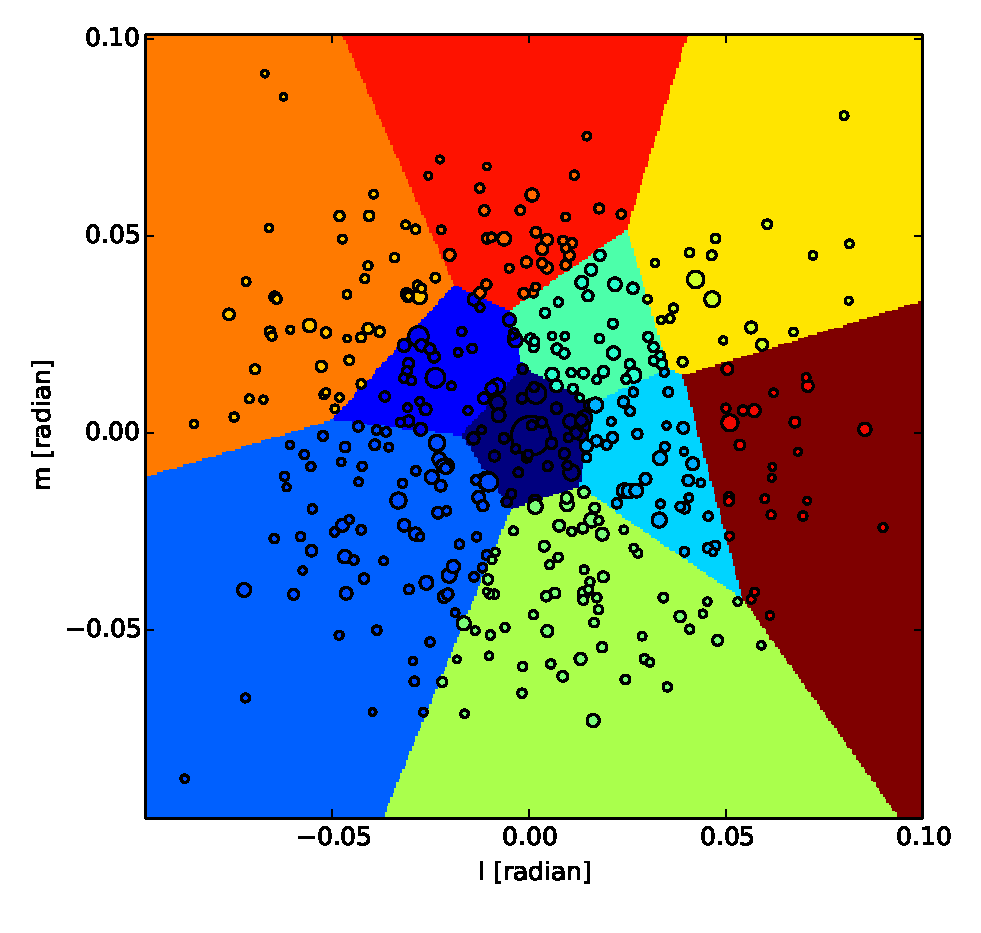
\includegraphics[width=8cm]{tessel}
\caption{\label{fig:tessel} In order to minimize the number of degrees
of freedom, and increase the amount of signal in each direction, we cluster the sources in 10 direction using a Voronoi
tesselation.}
\end{center}
\end{figure}


